\documentclass[10pt,utf8,presentation,notheorems,xcolor=dvipsnames,compress]{beamer}
\usepackage{doclad}

%Тут можно вставить дополнительные пакеты

\title[Базис Грёбнера]{
КАК КОМПЬЮТЕР ПОМОГАЕТ
УПРОЩАТЬ АЛГЕБРАИЧЕСКИЕ УРАВНЕНИЯ
}

\author[Блинков Ю.А.]{
 \href{http://www.sgu.ru/person/blinkov-yuriy-anatolevich}{Блинков~Юрий~Анатольевич}
}
\institute[РУДН, СГУ] {
Российский Университет Дружбы Народов (РУДН)\\
Руководитель научного центра вычислительных методов в прикладной математике
\vskip 5mm
«Саратовский национальный исследовательский\\ государственный университет имени Н.Г. Чернышевского»\\
зав. кафедрой «математического и компьютерного моделирования»
 
}
%%%%%%%%%%%%%%%%%%%%%%
\date{11 марта 2021}

\begin{document}

\begin{frame}
\titlepage
\end{frame}

\begin{frame}
Все исходные файлы доклада \url{https://github.com/blinkovua/Smart-Week}

\begin{block}{Допольнительные материалы}
Васильев Н. Н. КАК КОМПЬЮТЕР ПОМОГАЕТ УПРОЩАТЬ АЛГЕБРАИЧЕСКИЕ УРАВНЕНИЯ. Компьютерные инструменты в образовании. \\
\url{http://cte.eltech.ru/ojs/index.php/kio/article/view/964}
\vskip 5mm
Васильев Н. Н. УПРОЩЕНИЕ СИСТЕМЫ ПОЛИНОМИАЛЬНЫХ УРАВНЕНИЙ. Компьютерные инструменты в образовании.\\ 
\url{http://cte.eltech.ru/ojs/index.php/kio/article/view/970}
\end{block}
\end{frame}


\begin{frame}
5 января 2021 г. ушел из жизни Владимир Петрович Гердт, доктор физико-математических наук, профессор, начальник сектора алгебраических и квантовых вычислений Научного отдела вычислительной физики Лаборатории информационных технологий Объединенного института ядерных исследований, г. Дубна.
\begin{center}
\vskip -5mm
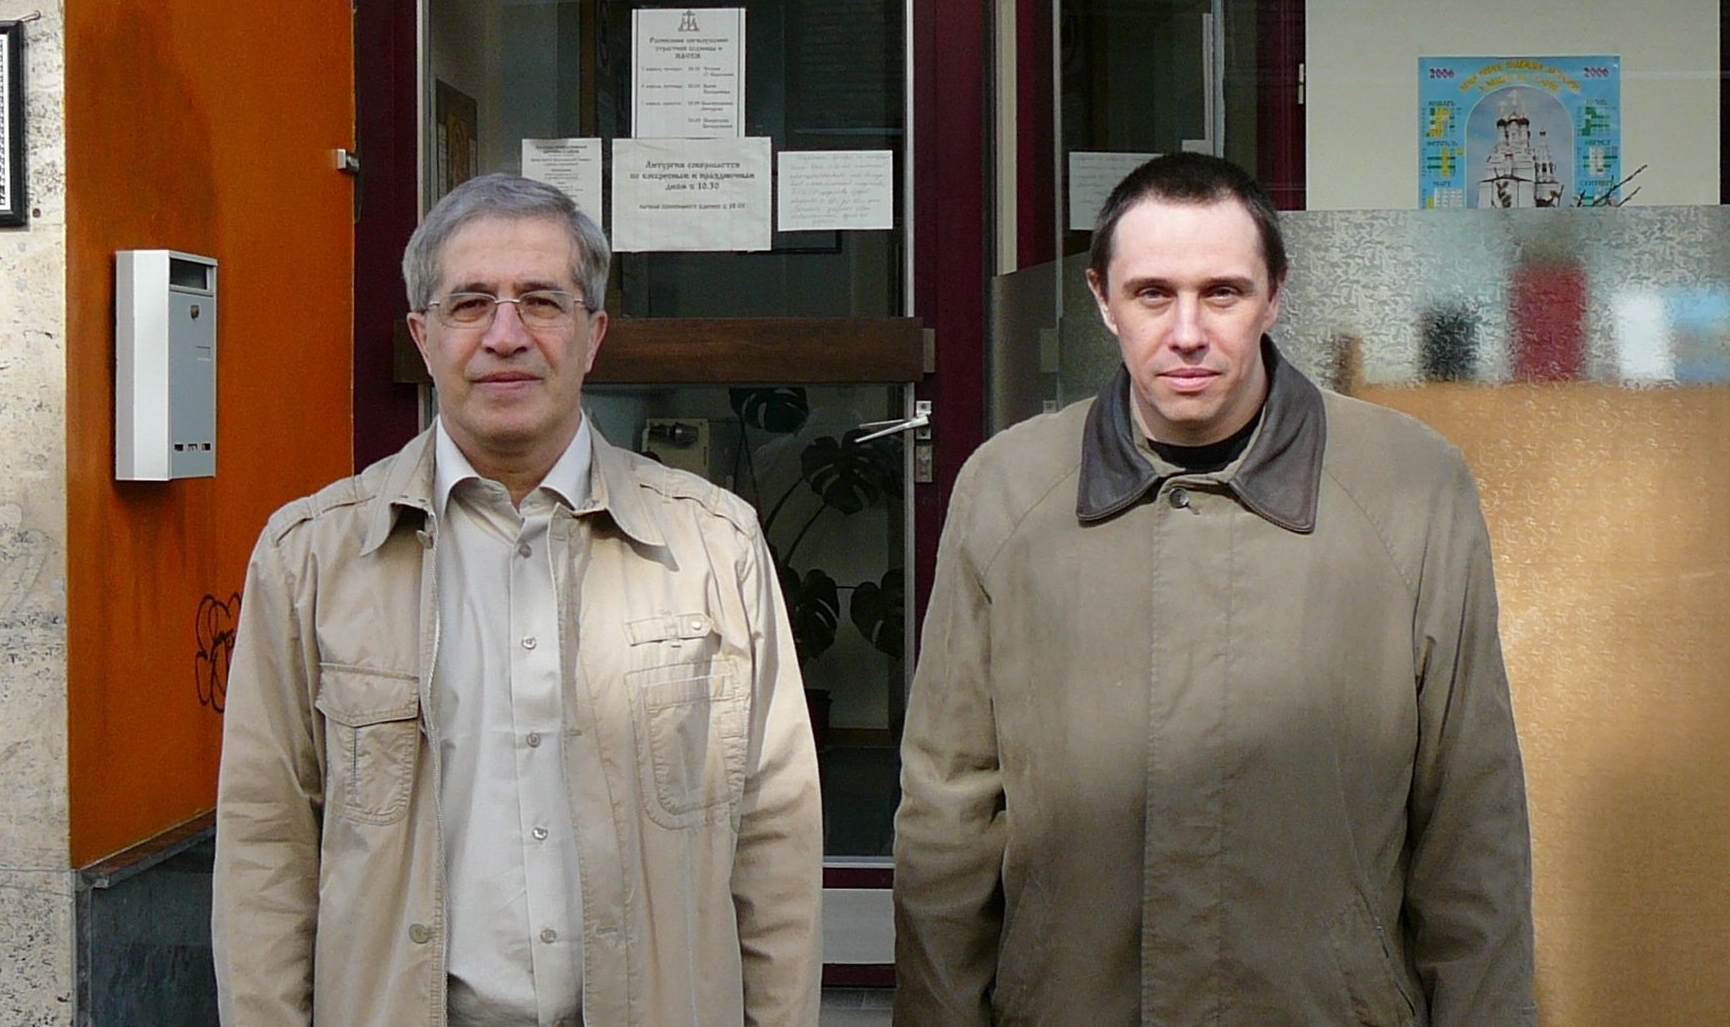
\includegraphics[height=.95\textheight]{p1000052.jpg}
\end{center}
\end{frame}


\begin{frame}[fragile]
\begin{Verbatim}[fontsize=\small,frame=leftline]
(*) --> "Ввод a, b, c"
"Ввод a, b, c" --> "D = b^2 - 4 a c"
if "D < 0" then
  -->[да] "Нет решения"
  --> (*)
else
  -->[нет] if "D = 0" then
	    -->[да] "Одно решение\nx = -b/(2 a)"
	    --> (*)
	  else
	    -->[нет] "Два решения\nx = (-b + D)/(2 a)\nx = (-b - D)/(2 a)"
	    --> (*)
	  endif
endif
\end{Verbatim}
\end{frame}

\begin{frame}
\begin{center}
\vskip -5mm
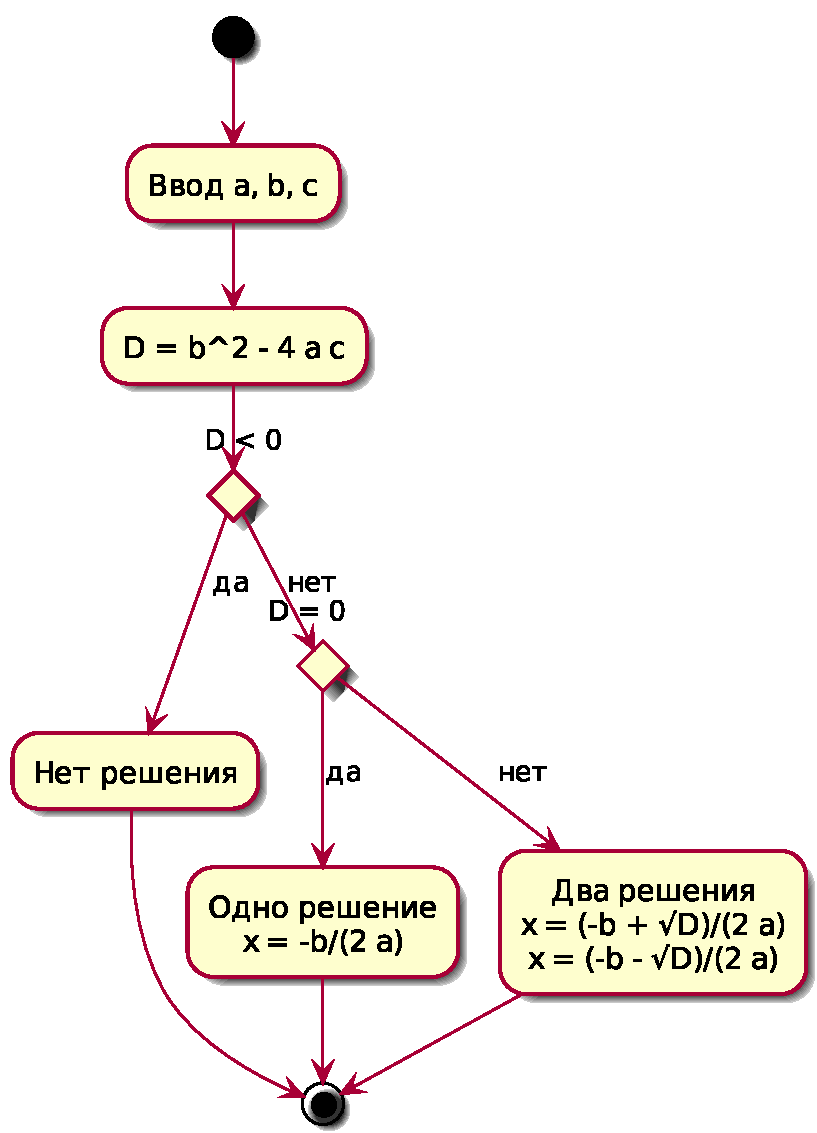
\includegraphics[height=.95\textheight]{Quadratic_equation}
\end{center}
\end{frame}

\begin{frame}
\begin{block}{Graphviz (сокращение от англ. Graph Visualization Software)}
пакет утилит по автоматической визуализации графов, заданных в виде описания на 
языке DOT, а также дополнительных TUI и GUI программ, виджетов и библиотек, 
используемых при разработке программного обеспечения для визуализации 
структурированных данных. Пакет Graphviz разработан специалистами лаборатории 
AT\&T и распространяется с открытыми исходными файлами по лицензии EPL (Eclipse 
Public License) и работает на многих операционных системах, включая Linux, Mac 
OS, Unix-подобные, Microsoft Windows.
\end{block}

\begin{center}
Сайт \href{http://graphviz.org/}{graphviz.org}
\end{center}
\end{frame}

\begin{frame}
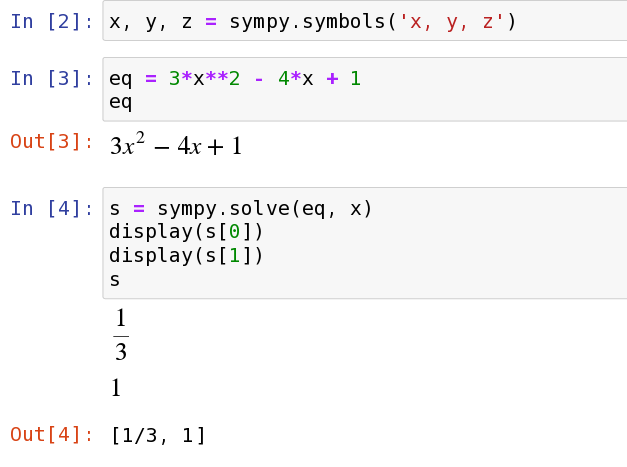
\includegraphics[width=.95\textwidth]{qe1.png}
\end{frame}

\begin{frame}
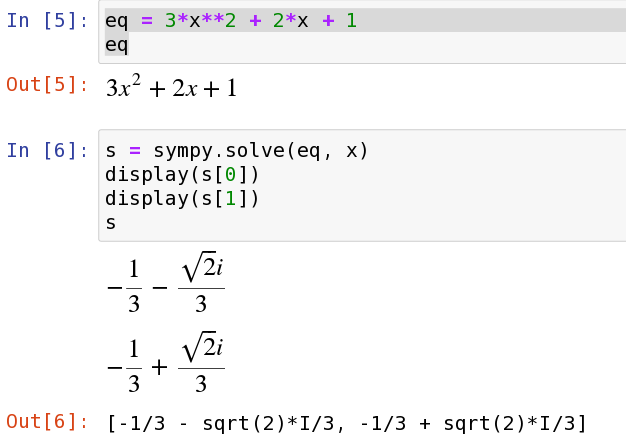
\includegraphics[width=.95\textwidth]{qe2.png}
\end{frame}

\begin{frame}
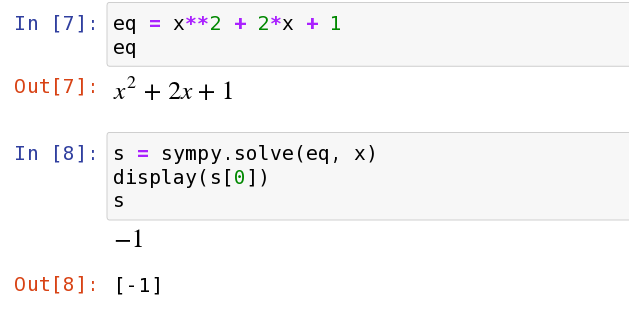
\includegraphics[width=.95\textwidth]{qe3.png}
\end{frame}

\begin{frame}
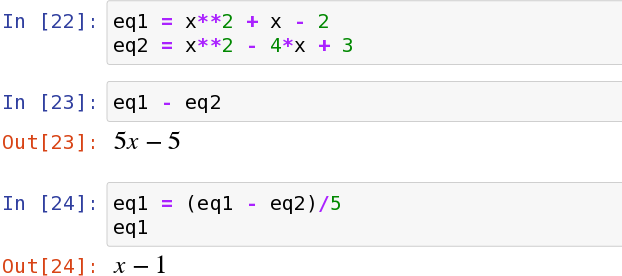
\includegraphics[width=.95\textwidth]{gcd11.png}
\end{frame}

\begin{frame}
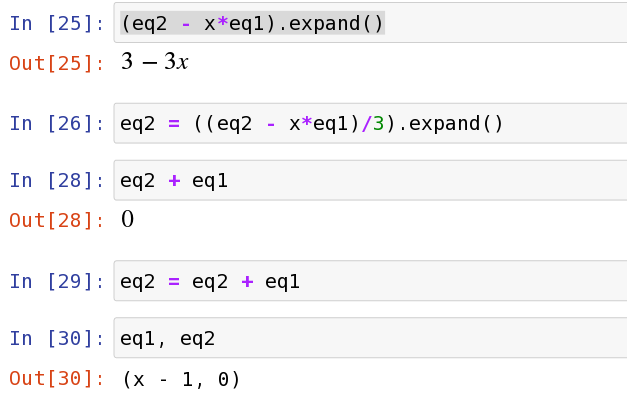
\includegraphics[width=.95\textwidth]{gcd12.png}
\end{frame}

\begin{frame}
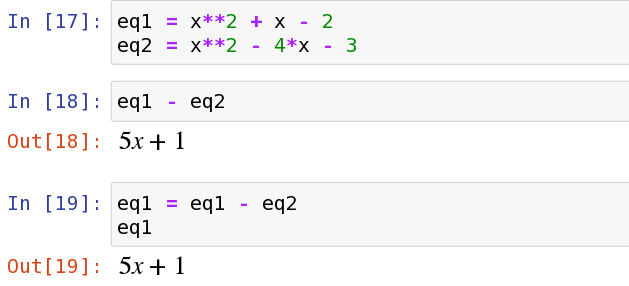
\includegraphics[width=.95\textwidth]{gcd21.png}
\end{frame}

\begin{frame}
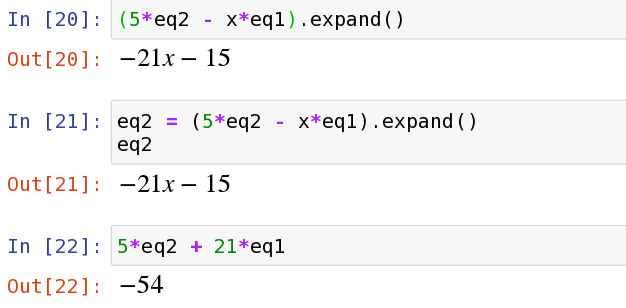
\includegraphics[width=.95\textwidth]{gcd22.png}
\end{frame}

\begin{frame}
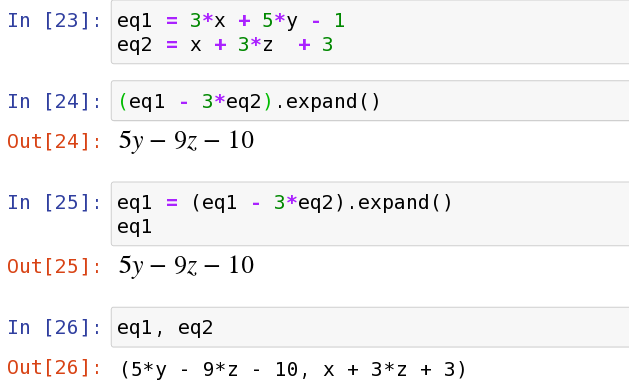
\includegraphics[width=.95\textwidth]{gaus.png}
\end{frame}


\begin{frame}
\begin{block}{Определение}
(Допустимым) мономиальным упорядочением на множестве мономов называется линейный порядок, 
удовлетворяющий следующим свойствам:
\begin{itemize}
\item для любого момома $a$ выполнено $1 \prec a$;
\item если $a \prec b$, то для любого $c$ выполнено $a\cdot c \prec b\cdot c$.
\end{itemize}
\end{block}

\begin{block}{Случай одной переменной}
Можно задать только один допустимый порядок --- по степени переменной:
$$x \prec x^2 \prec x^3 \prec x^4 \prec x^5 \prec x^6  \prec \ldots$$
\end{block}

\begin{block}{Случай нескольких переменных}
Сначала задают порядок переменных, например: $z \prec y \prec x$

Наиболее часто используют \emph{lex} и \emph{deglex}.

\emph{lex}: $z  \prec z^2  \prec \ldots \prec y \prec y\cdot z \prec y\cdot z^2
\prec \ldots\prec y^2 \prec y^2\cdot z  \prec y^2\cdot z^2
\prec \ldots\prec x \prec x\cdot z  \prec x\cdot z^2 \ldots \ldots\prec x\cdot y
\prec x\cdot y\cdot z \prec x\cdot y\cdot z^2 \prec \ldots$ 

\emph{deglex}: $z \prec y \prec x \prec z^2 \prec y\cdot z
 \prec y^2  \prec x\cdot z  \prec x\cdot y  \prec x^2  \prec z^3 \prec \ldots$ 
\end{block}
\end{frame}

\begin{frame}
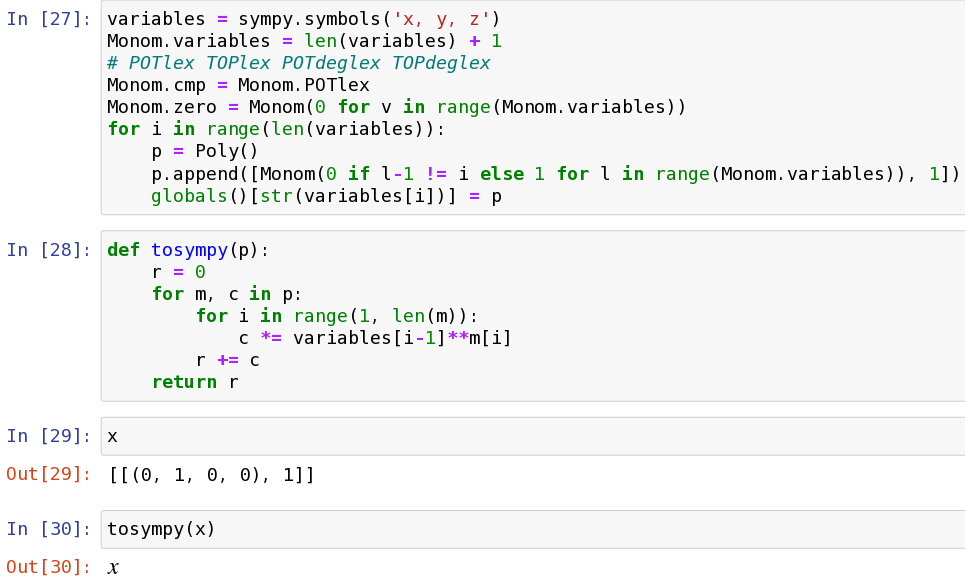
\includegraphics[width=1.04\textwidth]{gb1.png}
\end{frame}

\begin{frame}{\emph{lex}}
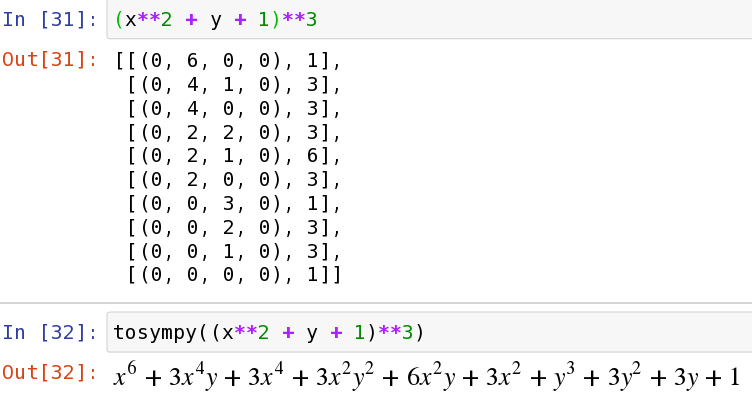
\includegraphics[width=1.0\textwidth]{gb2.png}
\end{frame}

\begin{frame}{\emph{deglex}}
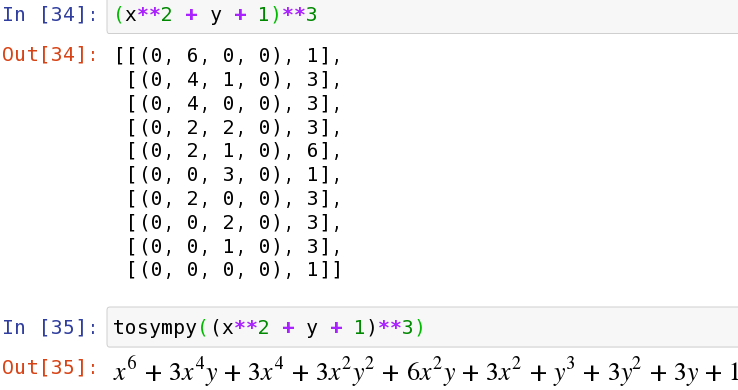
\includegraphics[width=1.0\textwidth]{gb3.png}
\end{frame}

\begin{frame}{\emph{deglex}}
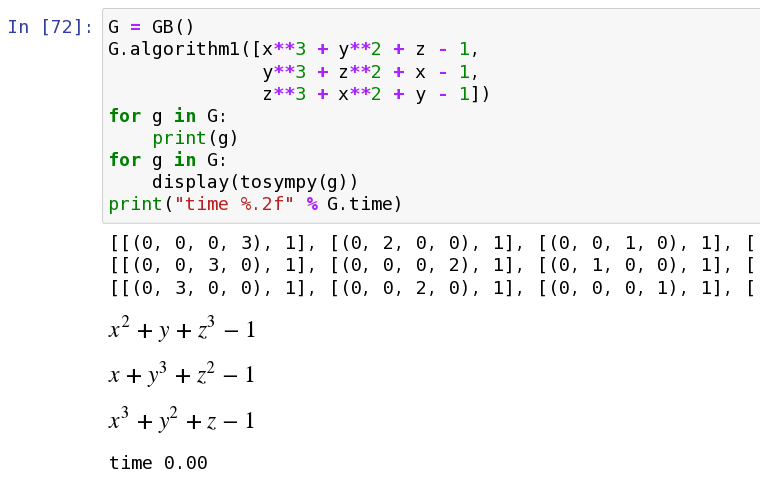
\includegraphics[width=1.0\textwidth]{gb4.png}
\end{frame}

\begin{frame}{\emph{lex}}
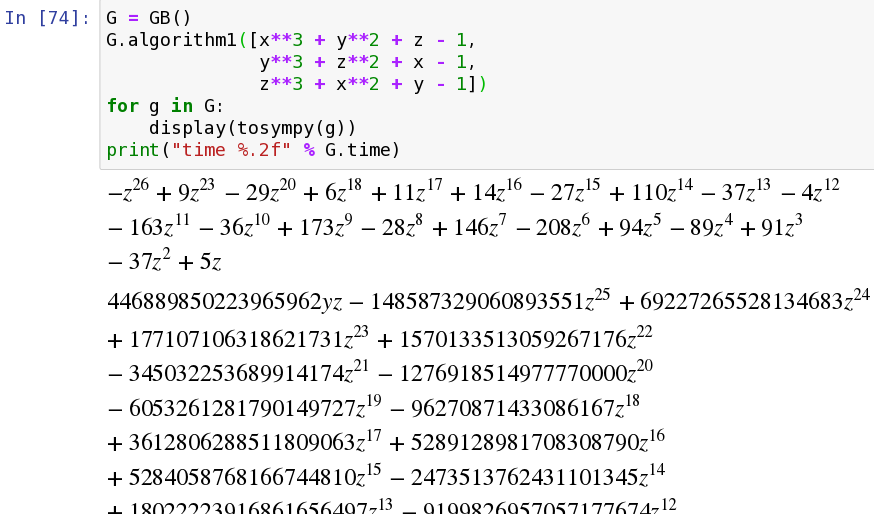
\includegraphics[width=1.0\textwidth]{gb51.png}
\end{frame}

\begin{frame}{\emph{lex}}
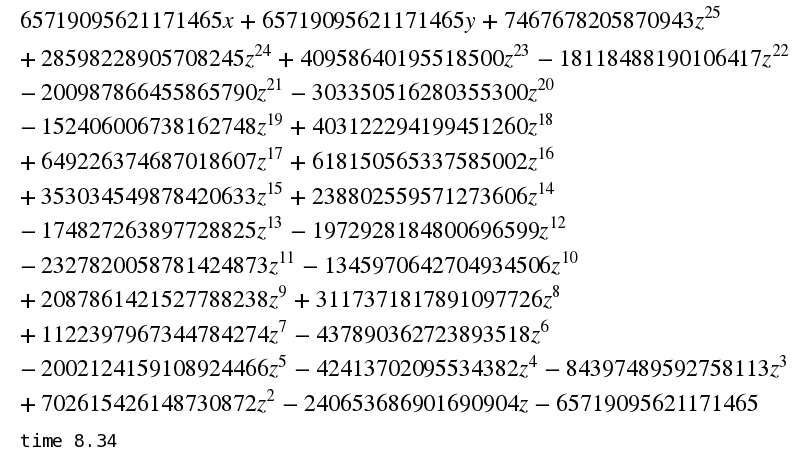
\includegraphics[width=1.0\textwidth]{gb52.png}
\end{frame}

\begin{frame}{\emph{lex}}
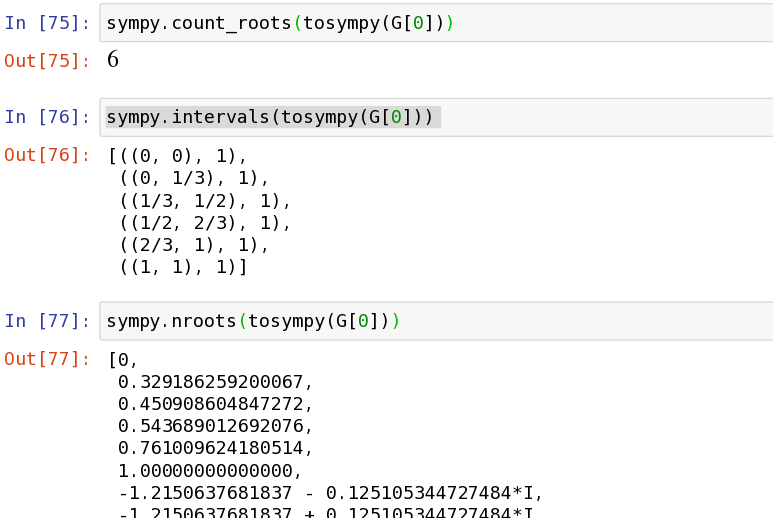
\includegraphics[width=1.0\textwidth]{gb53.png}
\end{frame}


\begin{frame}
\begin{block}{\emph{lex}: старшие члены $z^{27}, y, x$}
мономов без делителя на старшие члены $=27$
$$1_{\mathbb{M}}, z, z^2,  \ldots, z^{26}$$
\end{block}

\begin{block}{\emph{deglex}: старшие члены $z^3, y^3, x^3$}
мономов без делителя на старшие члены $=27$
$$1_{\mathbb{M}},=1$$ 
$$z, y, x,=3$$ 
$$z^2, yz, y^2, xz, xy, x^2,=6$$
$$yz^2, y^2z, xz^2, xyz, xy^2, x^2z, x^2y,=7$$
$$y^2z^2, xyz^2, xy^2z, x^2z^2, x^2yz, x^2y^2,=6$$
$$xy^2z^2, x^2yz^2, x^2y^2z,=3$$
$$x^2y^2z^2.=1$$
\end{block}
\end{frame}

\begin{frame}
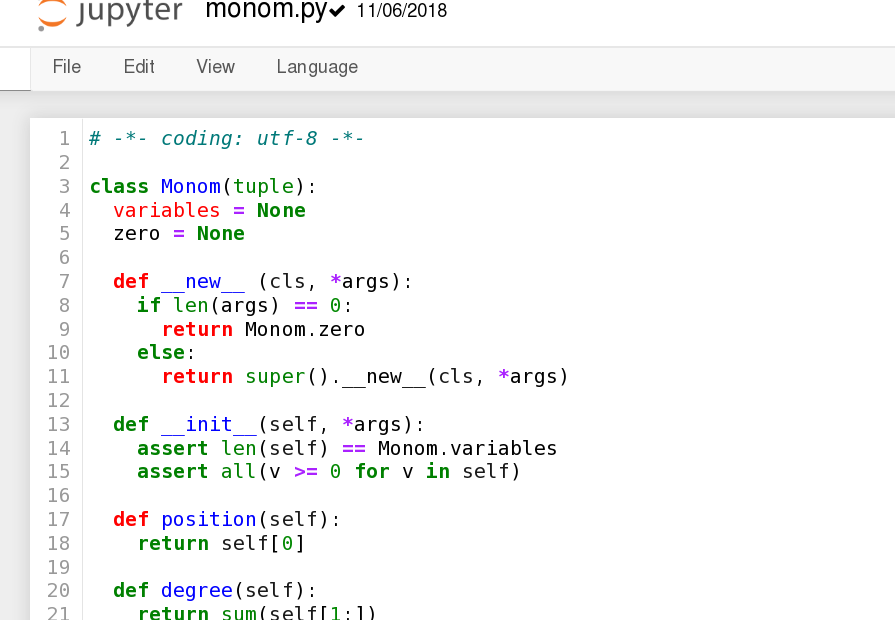
\includegraphics[width=0.9\textwidth]{monom.png}
\end{frame}

\begin{frame}
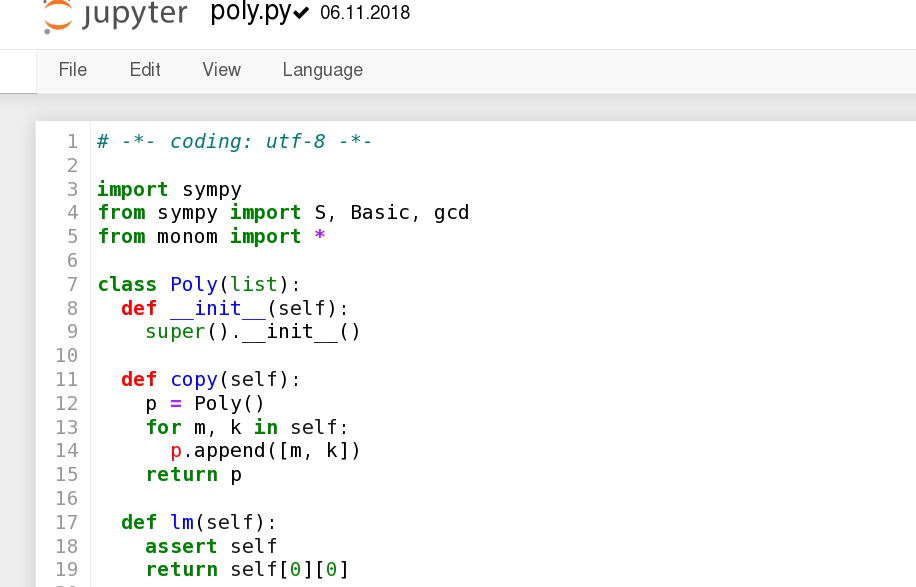
\includegraphics[width=0.9\textwidth]{poly.png}
\end{frame}

\begin{frame}{базис Грёбнера, алгоритм Бухбергера, инволютивный}
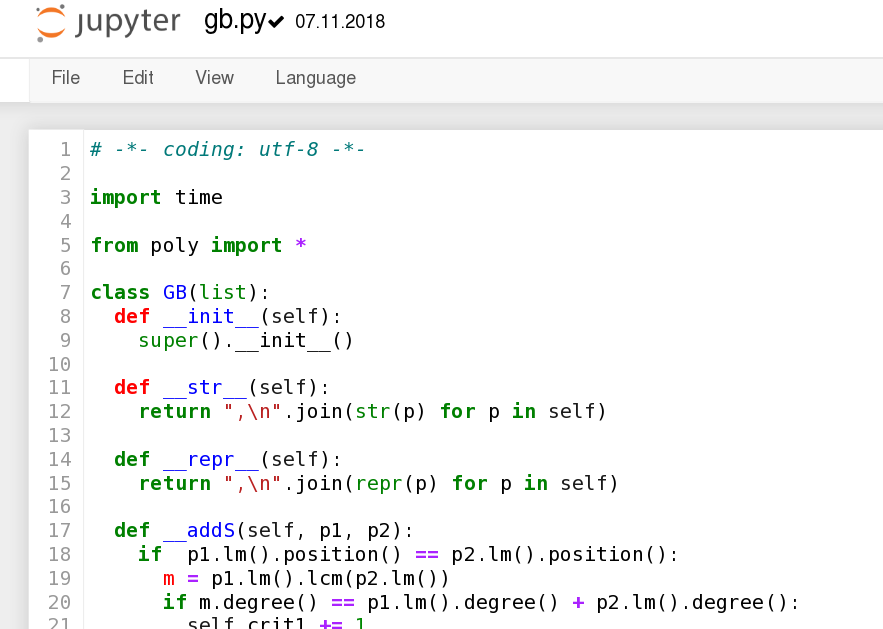
\includegraphics[width=0.9\textwidth]{gb.png}
\end{frame}

\begin{frame}{\url{https://www.sympy.org/en/index.html}}

\includegraphics[width=0.9\textwidth]{Sympy_logo.svg.png}
\end{frame}


\begin{frame}
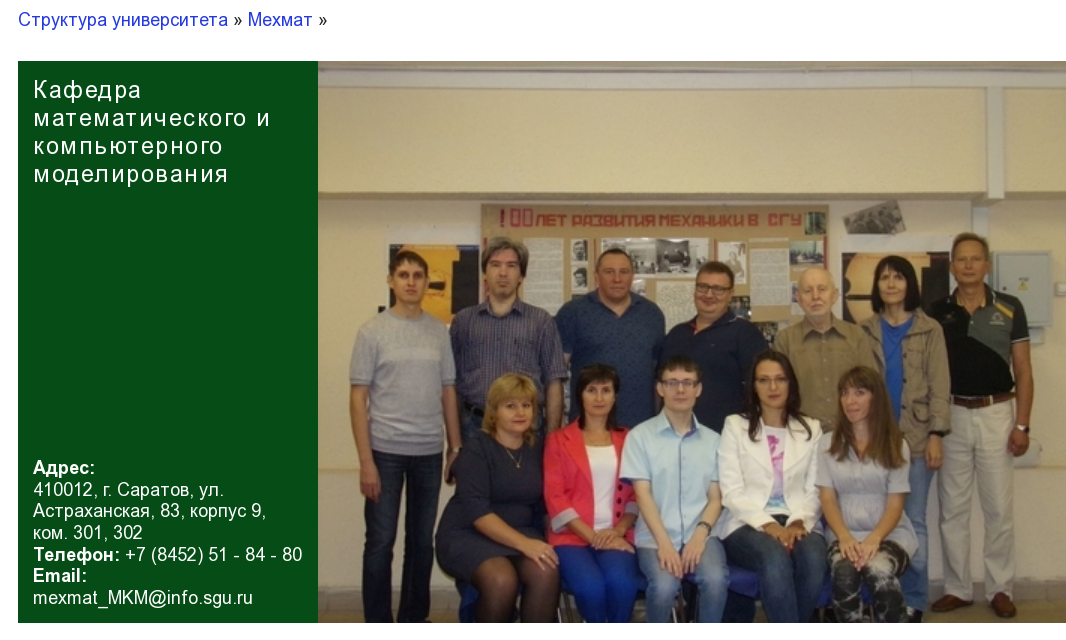
\includegraphics[width=1.0\textwidth]{MiKM.png}
\end{frame}

\begin{frame}
Все исходные файлы доклада \url{https://github.com/blinkovua/Smart-Week}

\begin{block}{Допольнительные материалы}
Васильев Н. Н. КАК КОМПЬЮТЕР ПОМОГАЕТ УПРОЩАТЬ АЛГЕБРАИЧЕСКИЕ УРАВНЕНИЯ. Компьютерные инструменты в образовании. \\
\url{http://cte.eltech.ru/ojs/index.php/kio/article/view/964}
\vskip 5mm
Васильев Н. Н. УПРОЩЕНИЕ СИСТЕМЫ ПОЛИНОМИАЛЬНЫХ УРАВНЕНИЙ. Компьютерные инструменты в образовании.\\ 
\url{http://cte.eltech.ru/ojs/index.php/kio/article/view/970}
\end{block}
\end{frame}

\end{document}



\begin{frame}[allowframebreaks]{Содержание}
\tableofcontents%[pausesections]
\end{frame}
